\chapter{Results}\label{ch:results}
We now describe the results of testing the ILP systems. 





%Q1 Does varying the quality of game traces influence the ability for learners to solve the IGGP problems? Specifically, does the quality of game play affect predictive accuracy?
%Q2 Does varying the amount of game traces influence the ability for learners to solve the IGGP problems? Specifically, does the quality of game play affect predictive accuracy?
%Q3 Can we improve the performance of a learner by mixing the quality of traces?



\section{Answering research questions}


\section{Results summary}


\ac{cut this - show specific plots for each experiment}
We present the conglomerated results in two forms. As a table and as a bar graph. The full results for each game and predicate learned are too lengthy to include in this paper. They can however be found in the code repository\footnote{https://github.com/Aflynn50/GPP-3rd-year-project} as well as by rerunning the experiment.


 \ac{I would reiterate the research questions here}

\ac{
	Are the results the same for all the games?
	Are their any games in particular that benefit from more traces or optimal play?
}

\subsection{E1: Varying the quality of game traces}
\ac{talk about the results of this experiment}



\ac{Table \ref{tab:e1results} shows the results of E1 ....}
We found that overall the systems trained on the mixed data did better than the systems trained on random data.
\ac{how much better?}
However the difference in score was not particularly pronounced \ac{what does that mean?}.

\ac{ILASP ...}

The Metagol system was ineffective across all sets of data. It sometime managed to learn part of the \textit{next} predicate for some games but never managed \textit{legal} or \textit{goal} predicates.

Aleph was limited by the maximum size of the program to be learned. This affected its performance on the larger number of traces. Aleph often did well at learning the \textit{goal} and \textit{next} predicates however was generally scored poorly on the more complex \textit{legal} predicate. The system did not do significantly better on optimal or random. It performed well when trained and tested on the Sancho traces.
The programs that were learned by the Aleph system almost always consisted of a conjunction of the examples in the training set. This method was only effective \ac{any idea why?}
\af{talk about info that cant be glended from the graph}


\subsection{E2: Varying the amount of game traces}
\af{use scatter graph}
\ac{talk about the results of this experiment}
\ac{
	I would present these as a scatter plot. On the xaxis you have the amount of game traces and on the y axis you have the balanced accuracy / perfectly scored metric
}


When increasing the number of traces it was observed that the there was a large jump in effectiveness of ILASP between 8 and 16 traces but between 16 and 24 traces the aggregated results were identical suggesting the new extra game traces had no benefit to the ILP systems. The number of games the ILASP perfectly solved also jumped by a huge amount, from 7-8 to 76 suggesting that this system in particular benefited a lot from the extra data.

\ac{What about Metagol?}

\ac{What about Aleph?}


\subsection{E3: Mixing the quality of traces}
\ac{talk about the results of this experiment}









Balanced accuracy

\begin{table}[]
	\begin{tabular}{|c|c|c|c|c|c|c|}
		\hline
		\multicolumn{7}{|c|}{Balanced Accuracy}                                                                           \\ \hline
		\multirow{2}{*}{Systems} & \multicolumn{2}{c|}{Random} & \multicolumn{2}{c|}{Sancho} & \multicolumn{2}{c|}{Mixed} \\ \cline{2-7}
		& Random       & Sancho       & Random       & Sancho       & Random       & Sancho      \\ \hline
		Metagol                  & 51           & 51           & 51           & 51           & 51           & 51          \\ \hline
		Aleph                    & 66           & 65           & 65           & 72           & 80           & 66          \\ \hline
		ILASP                    & 72           & 72           & 71           & 72           & 73           & 73          \\ \hline
	\end{tabular}
	\label{givemeaname}
	\caption{\ac{give me a caption - explain what the columns are. Which column / row is train? Which is test?}}
\end{table}


\begin{table}[]
	\begin{tabular}{|c|c|c|c|c|c|c|}
		\hline
		\multicolumn{7}{|c|}{Perfectly Solved}                                                                            \\ \hline
		\multirow{2}{*}{Systems} & \multicolumn{2}{c|}{Random} & \multicolumn{2}{c|}{Sancho} & \multicolumn{2}{c|}{Mixed} \\ \cline{2-7}
		& Random       & Sancho       & Random       & Sancho       & Random       & Sancho      \\ \hline
		Metagol                  & 0            & 0            & 0            & 0            & 0            & 0           \\ \hline
		Aleph                    & 1            & 0            & 0            & 4            & 7            & 0           \\ \hline
		ILASP                    & 7            & 8            & 5            & 10           & 7            & 8           \\ \hline
	\end{tabular}
	\label{givemeaname}
	\caption{\ac{give me a caption}}
\end{table}

\begin{table}[]
	\begin{tabular}{|c|c|c|c|c|c|c|}
		\hline
		\multicolumn{7}{|c|}{Balenced Accuracy}                                                                                       \\ \hline
		\multirow{2}{*}{Systems} & \multicolumn{2}{c|}{Mixed - 8} & \multicolumn{2}{c|}{Mixed - 16} & \multicolumn{2}{c|}{Mixed - 24} \\ \cline{2-7}
		& Random         & Sancho        & Random         & Sancho         & Random         & Sancho         \\ \hline
		Metagol                  & 51             & 51            & 51             & 51             & 51             & 51             \\ \hline
		Aleph                    & 67             & 66            & 67             & 65             & 67             & 65             \\ \hline
		ILASP                    & 73             & 73            & 85             & 85             & 85             & 85             \\ \hline
	\end{tabular}
	\label{givemeaname}
	\caption{\ac{give me a caption}}
\end{table}

\begin{table}[]
	\begin{tabular}{|c|c|c|c|c|c|c|}
		\hline
		\multicolumn{7}{|c|}{Perfectly Solved}                                                                                        \\ \hline
		\multirow{2}{*}{Systems} & \multicolumn{2}{c|}{Mixed - 8} & \multicolumn{2}{c|}{Mixed - 16} & \multicolumn{2}{c|}{Mixed - 24} \\ \cline{2-7}
		& Random         & Sancho        & Random         & Sancho         & Random         & Sancho         \\ \hline
		Metagol                  & 0              & 0             & 0              & 0              & 0              & 0              \\ \hline
		Aleph                    & 1              & 0             & 0              & 0              & 0              & 0              \\ \hline
		ILASP                    & 7              & 8             & 76             & 76             & 76             & 76             \\ \hline
	\end{tabular}
	\label{givemeaname}
	\caption{\ac{give me a caption}}
\end{table}

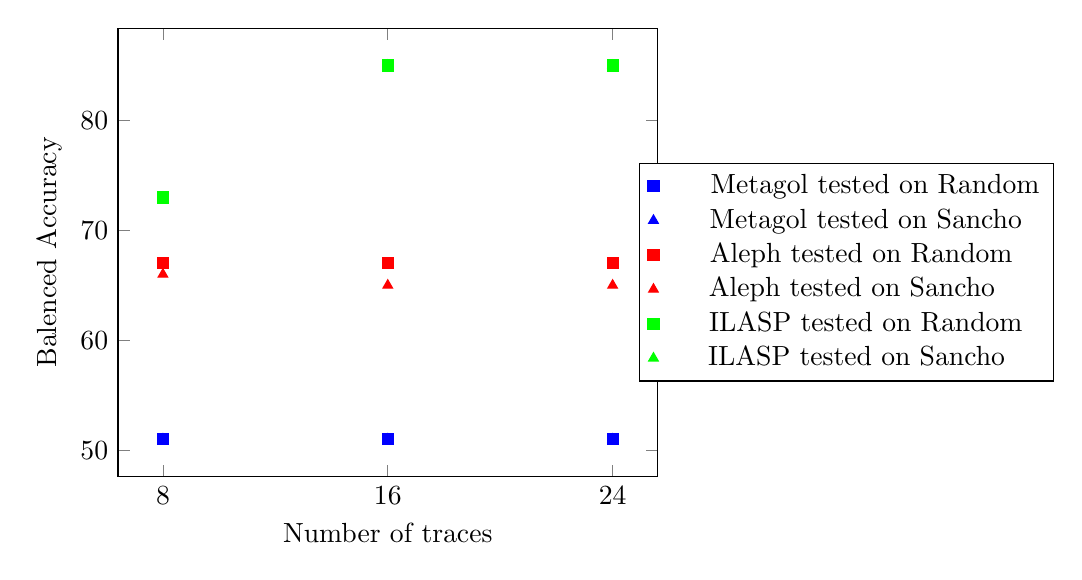
\begin{tikzpicture}
\begin{axis}[scatter/classes={
	a1={mark=square*,blue},%
	a2={mark=triangle*,blue},%
	b1={mark=square*,red},%
	b2={mark=triangle*,red},%
	c1={mark=square*,green},%
	c2={mark=triangle*,green}},
	legend style={at={(1.35,0.7)},
	anchor=north},
	xtick=data,
	ylabel={Balenced Accuracy},
	xlabel={Number of traces}]
\addplot[scatter,only marks,
	scatter src=explicit symbolic] coordinates {
	(8,51)     	[a1]
	(8,51)     	[a2]
	(16,51)    	[a1]
	(16,51)    	[a2]
	(24,51)    	[a1]
	(24,51)		[a2]
	(8,67)		[b1]
	(8,66)		[b2]
	(16,67)		[b1]
	(16,65)		[b2]
	(24,67)		[b1]
	(24,65)		[b2]
	(8,73)		[c1]
	(8,73)		[c2]
	(16,85)		[c1]
	(16,85)		[c2]
	(24,85)		[c1]
	(24,85)		[c2]
};
\legend{\ \ \ \ \ Metagol tested on Random,\ \ \ Metagol tested on Sancho,\ \ Aleph tested on Random,Aleph tested on Sancho, \ \ \ ILASP tested on Random,\ ILASP tested on Sancho,d}
\end{axis}

\end{tikzpicture}

\section{Varying quality training data}

\subsubsection{Random training}
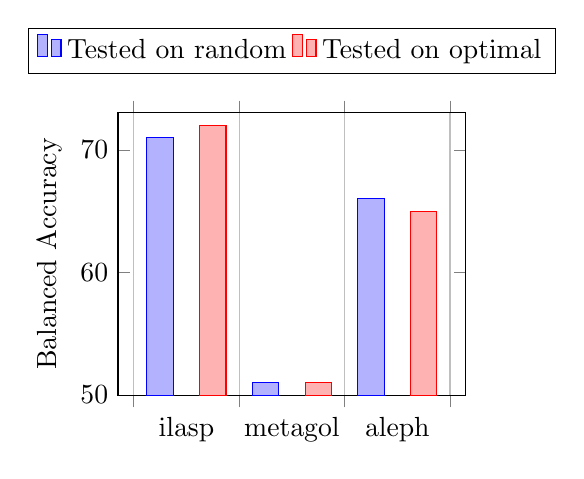
\begin{tikzpicture}
\begin{axis}[
	ylabel=Balanced Accuracy,
	width=6cm,
	enlargelimits=0.05,
	legend style={at={(0.5,1.3)},
	anchor=north,
	legend columns=-1},
	ybar interval=0.5,
	symbolic x coords={ilasp,metagol,aleph, poog}
]
\addplot
	coordinates {(ilasp,71) (metagol,51) (aleph,66) (poog, 65)};
\addplot
	coordinates {(ilasp,72) (metagol,51) (aleph,65) (poog,65)};
\legend{Tested on random,Tested on optimal}
\end{axis}
\end{tikzpicture}
~
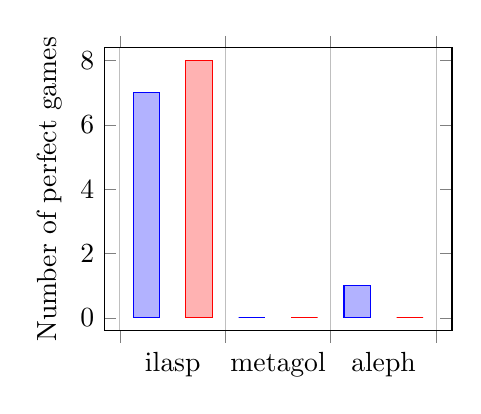
\begin{tikzpicture}
\begin{axis}[
	width=6cm,
	ylabel=Number of perfect games,
	enlargelimits=0.05,
	ybar interval=0.5,
	symbolic x coords={ilasp,metagol,aleph, poog}
]
\addplot
	coordinates {(ilasp,7) (metagol,0) (aleph,1) (poog, 0)};
\addplot
	coordinates {(ilasp,8) (metagol,0) (aleph,0) (poog,0)};
\end{axis}
\end{tikzpicture}
\subsubsection{Optimal training}
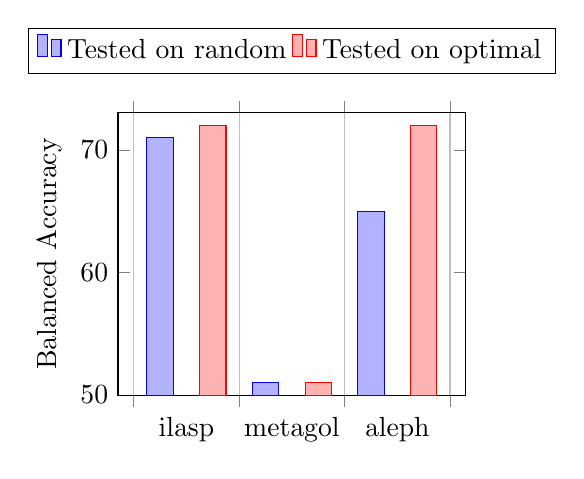
\begin{tikzpicture}
\begin{axis}[
ylabel=Balanced Accuracy,
width=6cm,
enlargelimits=0.05,
legend style={at={(0.5,1.3)},
	anchor=north,
	legend columns=-1},
ybar interval=0.5,
symbolic x coords={ilasp,metagol,aleph, poog}
]
\addplot
coordinates {(ilasp,71) (metagol,51) (aleph,65) (poog, 65)};
\addplot
coordinates {(ilasp,72) (metagol,51) (aleph,72) (poog,65)};
\legend{Tested on random,Tested on optimal}
\end{axis}
\end{tikzpicture}
~
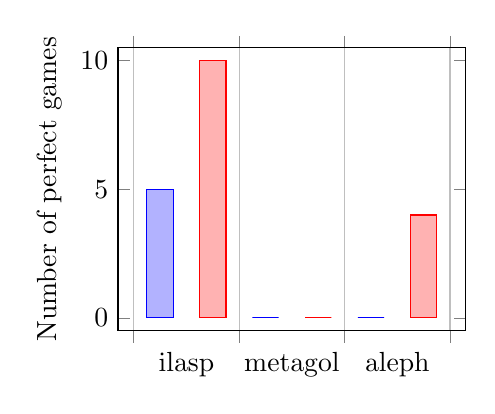
\begin{tikzpicture}
\begin{axis}[
width=6cm,
ylabel=Number of perfect games,
enlargelimits=0.05,
ybar interval=0.5,
symbolic x coords={ilasp,metagol,aleph, poog}
]
\addplot
coordinates {(ilasp,5) (metagol,0) (aleph,0) (poog, 0)};
\addplot
coordinates {(ilasp,10) (metagol,0) (aleph,4) (poog,0)};
\end{axis}
\end{tikzpicture}
\subsubsection{Mixed training}
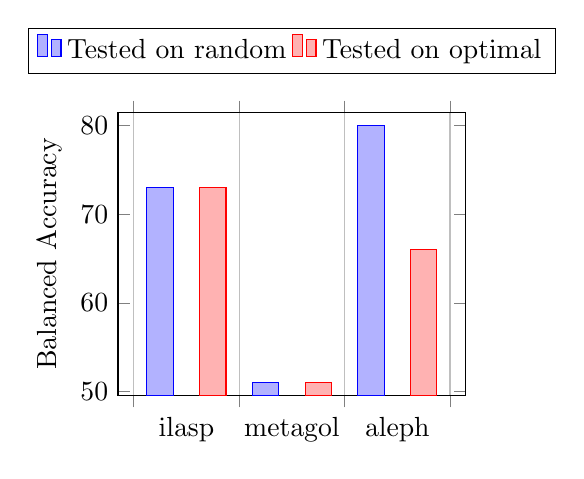
\begin{tikzpicture}
\begin{axis}[
ylabel=Balanced Accuracy,
width=6cm,
enlargelimits=0.05,
legend style={at={(0.5,1.3)},
	anchor=north,
	legend columns=-1},
ybar interval=0.5,
symbolic x coords={ilasp,metagol,aleph, poog}
]
\addplot
coordinates {(ilasp,73) (metagol,51) (aleph,80) (poog,70)};
\addplot
coordinates {(ilasp,73) (metagol,51) (aleph,66) (poog,70)};
\legend{Tested on random,Tested on optimal}
\end{axis}
\end{tikzpicture}
~
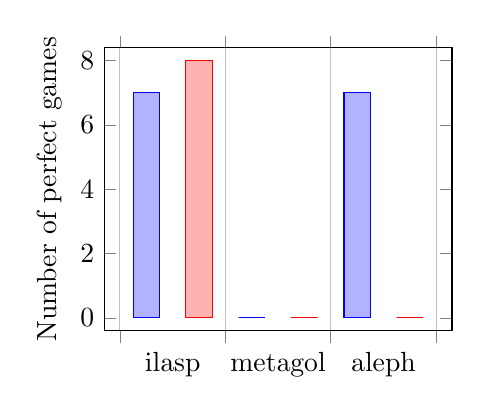
\begin{tikzpicture}
\begin{axis}[
width=6cm,
ylabel=Number of perfect games,
enlargelimits=0.05,
ybar interval=0.5,
symbolic x coords={ilasp,metagol,aleph, poog}
]
\addplot
coordinates {(ilasp,7) (metagol,0) (aleph,7) (poog, 0)};
\addplot
coordinates {(ilasp,8) (metagol,0) (aleph,0) (poog,0)};
\end{axis}
\end{tikzpicture}

\subsubsection{Mixed training with 16 traces}
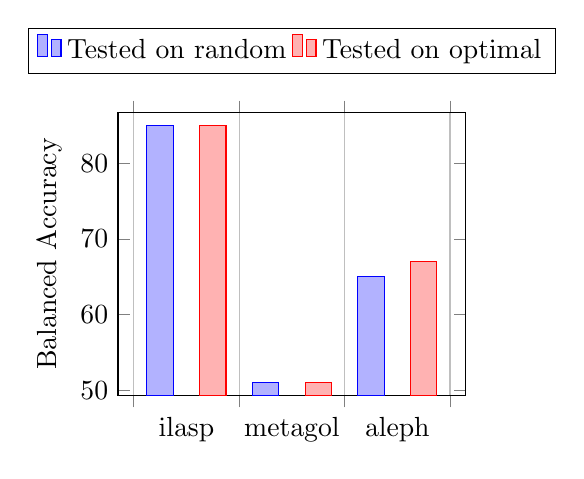
\begin{tikzpicture}
\begin{axis}[
ylabel=Balanced Accuracy,
width=6cm,
enlargelimits=0.05,
legend style={at={(0.5,1.3)},
	anchor=north,
	legend columns=-1},
ybar interval=0.5,
symbolic x coords={ilasp,metagol,aleph, poog}
]
\addplot
coordinates {(ilasp,85) (metagol,51) (aleph,65) (poog,70)};
\addplot
coordinates {(ilasp,85) (metagol,51) (aleph,67) (poog,70)};
\legend{Tested on random,Tested on optimal}
\end{axis}
\end{tikzpicture}
~
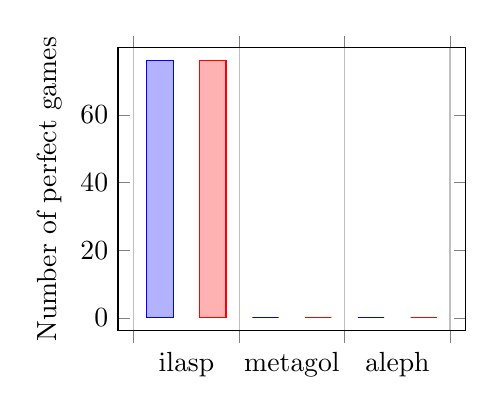
\begin{tikzpicture}
\begin{axis}[
width=6cm,
ylabel=Number of perfect games,
enlargelimits=0.05,
ybar interval=0.5,
symbolic x coords={ilasp,metagol,aleph, poog}
]
\addplot
coordinates {(ilasp,76) (metagol,0) (aleph,0) (poog, 0)};
\addplot
coordinates {(ilasp,76) (metagol,0) (aleph,0) (poog,0)};
\end{axis}
\end{tikzpicture}

\subsubsection{Mixed training with 24 traces}
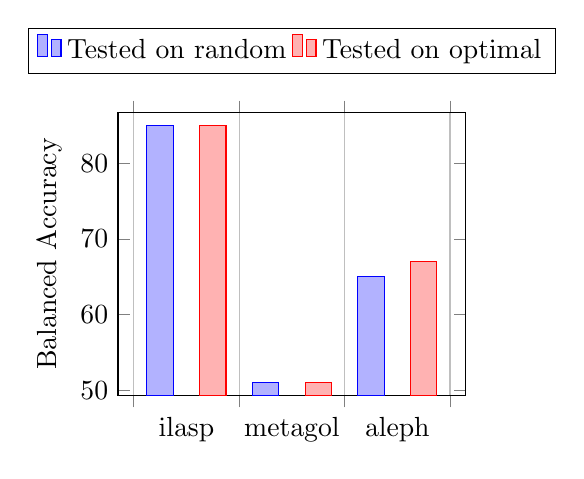
\begin{tikzpicture}
\begin{axis}[
ylabel=Balanced Accuracy,
width=6cm,
enlargelimits=0.05,
legend style={at={(0.5,1.3)},
	anchor=north,
	legend columns=-1},
ybar interval=0.5,
symbolic x coords={ilasp,metagol,aleph, poog}
]
\addplot
coordinates {(ilasp,85) (metagol,51) (aleph,65) (poog,70)};
\addplot
coordinates {(ilasp,85) (metagol,51) (aleph,67) (poog,70)};
\legend{Tested on random,Tested on optimal}
\end{axis}
\end{tikzpicture}
~
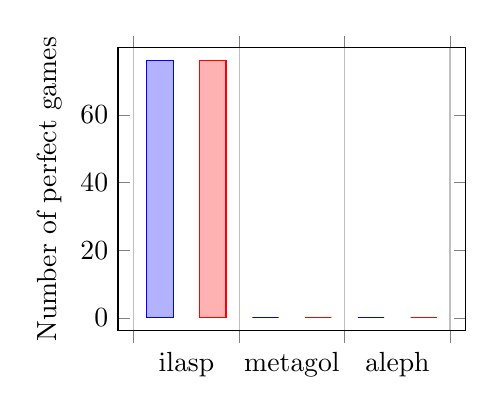
\begin{tikzpicture}
\begin{axis}[
width=6cm,
ylabel=Number of perfect games,
enlargelimits=0.05,
ybar interval=0.5,
symbolic x coords={ilasp,metagol,aleph, poog}
]
\addplot
coordinates {(ilasp,76) (metagol,0) (aleph,0) (poog, 0)};
\addplot
coordinates {(ilasp,76) (metagol,0) (aleph,0) (poog,0)};
\end{axis}
\end{tikzpicture}

